\documentclass[]{article}

\usepackage{proceed2e}
\usepackage{times}
\usepackage{helvet}
\usepackage{courier}
\usepackage{amsmath}
\usepackage{amsfonts}
\usepackage[vlined,algoruled,titlenumbered,noend,oldcommands]{algorithm2e}
\usepackage{graphicx}
\usepackage{caption}
\usepackage{multirow}
\usepackage{subcaption}
\usepackage{enumitem}
\usepackage{authordate1-4}
%\usepackage{natbib}

\setlength{\pdfpagewidth}{8.5in} 
\setlength{\pdfpageheight}{11in}

% if you are using PDF LaTex and you cannot find a way for producing
% letter, the following explicit settings may help
\newcommand{\contmax}{\mathrm{max}}
\newcommand{\casemax}{\mathrm{casemax}}
\newcommand{\casemin}{\mathrm{casemin}}

%\everymath{\displaystyle}

\begin{document}

\title{Closed-form Solutions to a Subclass of Continuous Stochastic Games via Symbolic Dynamic Programming}

%\numberofauthors{1}

%\author{
%\alignauthor
%XXX
%}

\maketitle

%-----------------------------------------------------------------------------
% Abstract
%-----------------------------------------------------------------------------

The binary (two-class) classification problem is an important subclass
of the classification problem in supervised machine learning. Its task
is to split the input space into two sides, namely ``yes'' -- ``no'',
or ``true'' -- ``false''. Examples include testing for a certain
disease, or testing if a critical component has failed. The direct and
most natural way to solve this problem is to minimize the 0--1 loss
function, which is the sum of classification errors in the training
data. However, 0--1 loss is highly non-convex and NP--hard to optimize
directly. Most of the existing algorithms, including support vector
machine (SVM), logistic regression, solve this problem using a
surrogate of the 0--1 loss function that is convex, and are hence
easily optimized. Although very successful, these algorithms are known
to suffer from the presence of outliers. In fact, all convex losses
suffer from outliers, while 0--1 loss does not. Therefore, the purpose
of this thesis is to study different approaches to direct optimization
of 0--1 loss for linear binary classification. For this purpose, four
anytime algorithms are proposed.  Numerous comparisons on synthetic
and real-world datasets with other state-of-the-art algorithms, such
as logistic regression, SVM, Bayes point machine, show that the novel
algorithms are almost always better, or at least comparable with
existing algorithms regarding 0--1 loss optimization. Importantly, in
the presence of outliers, the novel algorithms have a clear advantage
over all existing algorithms.









%-----------------------------------------------------------------------------
% Introduction
%-----------------------------------------------------------------------------

\section{Introduction}
%-----------------------------------------------------------------------------
%  What is the problem
%  Why is it interesting
%  What are your contributions
%  What is the outline
%-----------------------------------------------------------------------------

Modelling competitive sequential interactions between agents has 
important applications within economics and decision making. 
Stochastic games \cite{Shapley_PotNAoS_1953} provide a convenient framework 
to model sequential interactions between non-cooperative agents. In 
zero-sum stochastic games participating agents have diametrically 
opposing goals. A reinforcement learning solution to zero-sum stochastic
games with discrete states was presented by Littman \cite{Littman_ICML_1994}.
Closed form solutions for the continuous state case, however, remain unknown. 
Zero-sum continuous state stochastic games provide a convenient framework with 
which to model many important financial and economic domains, such 
as option valuation on derivative markets.

The difficulty of solving zero-sum continuous state stochastic games
arises from the need to calculate a Nash equilibrium for every state,
of which there are infinitely many. In this paper we characterise a subclass of 
continuous state stochastic games for which we can calculate exact solutions
via Symbolic dynamic programming (SDP)  \cite{Boutilier_IJCAI_2001},
for arbitrary horizons.

We begin by presenting Markov Decision Processes (MDPs) \cite{Howard_1960} 
and value iteration \cite{Bellman_1957}, a commonly used dynamic programming
solution for MDPs. We then describe both discrete and continuous state 
zero-sum stochastic games as game-theoretic generalisations of the MDP framework. 
Following this we show how symbolic dynamic programming
can be used to calculate the first known exact solution to a particular subclass of 
zero-sum continuous stochastic games. We conclude by calculating
exact solutions to continuous state matching pennies and a binary
option valuation game.

In this paper we make the following unique contributions:
\begin{itemize}
  \item   We characterise a subclass of zero-sum continuous stochastic games
            with restricted reward and transition functions that can be solved exactly
            via parameterised linear optimisation.
  \item  We provide an algorithm that solves this subclass of stochastic games exactly and 
            optimally using symbolic dynamic programming for arbitrary horizons.
\end{itemize}

%The key insight of this paper lies within the characterisation of a subclass
%of zero-sum continuous state stochastic games with restricted reward
%functions that can be solved via parameterised linear optimisation. We 
%show that this particular subset of games can be solved both symbolically and optimally
%for arbitrary horizons.


%-----------------------------------------------------------------------------
% MDPs 
%-----------------------------------------------------------------------------

\section{Markov Decision Processes}
\label{sec:mdp}

A Markov Decision Process (MDP) \cite{Howard_1960} is defined by the tuple
$ \left\langle S, A, T, R, h, \gamma \right\rangle$. $S$ and $A$ 
specify a finite set of states and actions, respectively.
$T$ is a transition function $T : S \times A \rightarrow S$ which 
defines the effect of an action on the state. $R$ is the
reward function $R : S \times A \rightarrow \mathbb{R}$ which 
encodes the preferences of the agent. The horizon $h$ represents the 
number of decision steps until termination and the discount factor $\gamma$ 
is used to discount future rewards. In general, an agent's objective is 
to find a policy, $\pi : S \rightarrow A$, which maximises the expected 
sum of discounted rewards over horizon $h$.

Value iteration \cite{Bellman_1957} is a general dynamic programming 
algorithm used solve MDPs. For each horizon $h$, two functions form 
the basis of the algorithm: $V^{h}(s)$, the value of state $s$, and 
$Q^{h}(s, a)$, the value of taking action $a$ in state $s$. The two 
functions satisfy the following recursive relationship:
\begin{align}
  Q^{h}(s, a) &= R(s, a) + \gamma \sum_{s' \in S} T(s, a, s') V^{h-1}(s') \\
  V^{h}(s) &= \max_{a \in A} Q^{h}(s, a).
\end{align}

The algorithm is executed by first initialising $V^{0}$  to $R(s, a)$. 
Then for each $h$, the value function for $V^{h}(s)$ is calculated from $V^{h-1}(s)$
until the intended $h$-stage-to-go value function is computed.
Value iteration converges linearly in the number of iterations to the true
values of $Q(s, a)$ and $V(s)$ \cite{Bertsekas_1987}.

MDPs can be used to model multiagent systems under the assumption 
that other agents are part of the environment and have fixed behaviour. 
As a result, they ignore the difference between responsive agents and 
a passive environment \cite{Hu_ICML_1998}. In the next section we 
present a game theoretic framework which generalises MDPs to 
situations with two or more agents.

%-----------------------------------------------------------------------------
% Markov Games with Discrete State
%-----------------------------------------------------------------------------

\section{Zero-sum Discrete Stochastic Games}
\label{sec:dsg}
Discrete state stochastic games (DSGs) are formally defined by the tuple
$ \left\langle S, A_{1}, \ldots, A_{n}, T, R_{1}, \ldots, R_{n}, h, \gamma\right\rangle$.
$S$ is a set of discrete states and $A_i$ is the action set available to agent 
$i$. T is a transition function $T : S \times A_1 \times \ldots \times A_n \rightarrow \Delta(S)$, 
where $\Delta(S)$ is the set of probability distributions over the state space $S$. 
The reward function $R_i : S \times A_1 \times \ldots \times A_n \rightarrow \mathbb{R}$ 
encodes the individual preferences of agent $i$. The horizon $h$ represents the 
number of decision steps until termination and the discount factor $\gamma \in [0, 1)$ 
is used to discount future rewards. In general, an agent's objective is 
to find a policy, $\pi_i : S \rightarrow \sigma_i(A_i)$ which maximises the expected 
sum of discounted rewards over horizon $h$. Here $\sigma_i(A_i)$ specifies
probability distributions over action set $A_i$. The optimal policy in a 
DSG may be stochastic, that is, it may define a mixed strategy for each state. 

%The goal of each agent in a stochastic game is to maximise its expected 
%discounted future rewards.

%Two agent zero-sum DSGs impose a condition on the reward structure 
%of the game whereby the goals of an agent and its opponent are diametrically
%opposed to one another. Under this restriction the reward structure can 
%be represented by a single reward function. The opponent's
%reward function is simply the opposite of the agent's. 
%Within this game 
%each agent attempts to maximise its expected discounted future rewards 
%in the minimax sense. Since the reward structure is zero-sum it is sufficient to view the 
%opponent as acting to minimise the agent's return.

Zero-sum DSGs are a type of DSG involving two agents with diametrically
opposing goals. Under these conditions the reward structure for the 
game can be represented by a single reward function since an agents
reward function is simply the opposite of their opponent's. The objective
of each agent is to maximise its expected discounted future rewards 
in the minimax sense. That is, each agent views its opponent as
acting to minimise the agent's reward. Zero-sum DSGs can be solved 
using a technique analogous to value iteration for MDPs \cite{Littman_ICML_1994}. 
The value function, $V^{h}(s)$, in this setting can be defined as:

{\small
\abovedisplayskip=0pt
\belowdisplayskip=0pt
\begin{equation}
\label{eq:dsgvfunc}
  V^{h}(s) = \max_{m_{a_{1}} \in \sigma_1(A_1)}\min_{m_{a_{2}} \in \sigma_2(A_2)} \sum_{a_1 \in A_1} \sum_{a_2 \in A_2} Q^{h}(s, a_1, a_2) \cdot m_{a_{1}} \cdot m_{a_{2}}
\end{equation}
}%

where $m_{a_i}$ is a mixed strategy from $\sigma_i(A_i)$. 
$Q^{h}(s, a_1, a_2)$, the quality of taking action $a_1$ against action $a_2$ in state $s$,
is given by:

{\small 
\abovedisplayskip=0pt
\belowdisplayskip=0pt
\begin{eqnarray}
\label{eq:dsgdiscqfunc}
  Q^{h}(s, a_1, a_2) &=& R(s, a_1, a_2) + \nonumber \\
  && \gamma \cdot \sum_{s' \in S} T(s, a_1, a_2, s') \cdot V^{h-1}(s').
\end{eqnarray}
}%

%It is well known that Equation \eqref{eq:dsgvfunc} can be further simplified to:
Equation \eqref{eq:dsgvfunc} can be further simplified by noting that
since the $\text{min}$ operation is ``inside'' the $\text{max}$, the minimum is achieved
for a deterministic action choice. This observation leads to the following
form:
{\small 
\abovedisplayshortskip =100pt
\belowdisplayshortskip =0pt
\begin{equation}
\label{eq:dsgvfunccompact}
  V^{h}(s) = \max_{m_{a_{1}} \in \sigma_1(A_1)} \min_{a_2 \in A_2} \sum_{a_1 \in A_1} Q^{h}(s, a_1, a_2) \cdot m_{a_1}.
\end{equation}
}%

Together Equations \eqref{eq:dsgdiscqfunc} and \eqref{eq:dsgvfunccompact}
define a recursive method to calculate the optimal solution to zero-sum
DSGs. The policy for the opponent can be calculated by applying symmetric
reasoning and the Minimax theorem \cite{Neumann_MA_1928}. 

\subsection{Solution Techniques}
\label{subsec:dsgsolution}

Zero-sum DSGs can be solved via discrete linear optimisation. The value
function in Equation \eqref{eq:dsgvfunccompact} can be reformulated as a linear
program through the following steps:

\begin{enumerate}
  \item Define $V^h(s)$ to be the value of the inner minimisation term in
            Equation \eqref{eq:dsgvfunccompact}. This leads to the following linear program for a known state $s$:
{\small
\abovedisplayskip=10pt
\belowdisplayskip=0pt 
\begin{subequations}
\begin{align}
&\text{maximise}   \  V^{h}(s) \nonumber \\
&\text{subject to}   \nonumber \\
&\  V^{h}(s) = \min_{a_2 \in A_2} \sum_{a_1 \in A_1} Q^{h}(s, a_1, a_2) \cdot m_{a_{1}} \label{eq:dsglpconstraint1} \\
                          &\  \sum_{a_{1} \in A_1} m_{a_{1}} = 1 ; \  m_{a_{1}} \geq 0 \qquad \forall a_{1} \in A_1 \nonumber
\end{align}
\end{subequations}
}%

  \item Replace the equality (=) in constraint \eqref{eq:dsglpconstraint1} with
  $\leq$ by observing that the maximisation of $V^{h}(s)$
  effectively pushes the $\leq$ condition to the = case. This gives: 
{\small 
\abovedisplayskip=8pt
\belowdisplayskip=0pt
\begin{subequations}
\begin{align}
&\text{maximise}   \  V^{h}(s) \nonumber \\
&\text{subject to}   \nonumber \\
&\  V^{h}(s) \leq \min_{a_2 \in A_2} \sum_{a_1 \in A_1} Q^{h}(s, a_1, a_2) \cdot m_{a_{1}} \label{eq:dsglpconstraint2} \\
                          &\  \sum_{a_{1} \in A_1} m_{a_{1}} = 1 ; \  m_{a_{1}} \geq 0 \qquad \forall a_{1} \in A_1 \nonumber
\end{align}
\end{subequations}
}%
  
  \item Remove the minimisation operator in constraint \eqref{eq:dsglpconstraint2}
            by noting that the minimum of a set is less than or equal to the minimum of all elements in the set.
            This leads to the final form of the discrete linear optimisation problem:
{\small 
\abovedisplayskip=8pt
\belowdisplayskip=0pt
\begin{align*}
&\text{maximise}   \  V^{h}(s) \nonumber \\
&\text{subject to}   \nonumber \\
&\  V^{h}(s) \leq \sum_{a_1 \in A_1} Q^{h}(s, a_1, a_2) \cdot m_{a_{1}} \ \forall a_2 \in A_2\\
                          &\  \sum_{a_{1} \in A_1} m_{a_{1}} = 1 ; \  m_{a_{1}} \geq 0 \qquad \forall a_{1} \in A_1 \nonumber
\end{align*}
}%
\end{enumerate}

We can now use existing linear programming solvers to compute the optimal
solution to this linear program for each $s \in S$ at a given horizon $h$.

The linear program used to solve zero-sum DSGs cannot be used once
the state is continuous since there are infinitely many states. The key 
innovation of this paper is in showing that continuous state zero-sum
games can still be solved through the use of symbolic dynamic programming.

%-----------------------------------------------------------------------------
% Markov Games with Continuous State
%-----------------------------------------------------------------------------

\section{Zero-sum Continuous Stochastic Games}
\label{sec:csg}

Continuous state stochastic games (CSGs) are formally defined by the tuple
$ \left\langle \vec{x}, A_{1}, \ldots, A_{n}, T, R_{1}, \ldots, R_{n}, h, \gamma  \right\rangle$.
In CSGs states are represented by vectors of continuous variables, $\vec{x} = \left(x_1, \ldots, x_m \right)$, 
where $x_i \in \mathbb{R}$. The other components of the tuple are as 
previously defined for discrete stochastic games in the preceding section.

The optimal solution to zero-sum CSGs can be calculated via the 
following recursive functions:
{\small 
\begin{eqnarray}
\label{eq:csgdiscqfunc}
  Q^{h}(\vec{x}, a_1, a_2) &=& R(\vec{x}, a_1, a_2) \quad + \nonumber \\
  && \gamma \cdot \int T(\vec{x}, a_1, a_2, \vec{x}') \cdot V^{h-1}(\vec{x}') d\vec{x}' 
\end{eqnarray}
}%

{\small 
\begin{equation}
\label{eq:csgvfunccompact}
  V^{h}(\vec{x}) = \max_{m_{a_{1}} \in \sigma(A_1)} \min_{a_2 \in A_2} \sum_{a_1 \in A_1} Q^{h}(\vec{x}, a_1, a_2) \cdot m_{a_{1}}
\end{equation}
}%

We can derive Equation \eqref{eq:csgdiscqfunc} from Equation \eqref{eq:dsgdiscqfunc}
by replacing the $s$, $s'$ and the $\sum$ operator with their continuous
state counterparts, $\vec{x}$, $\vec{x}'$ and $\int$, respectively.
%
%Here we note that Equation \eqref{eq:csgdiscqfunc} can be derived from Equation \eqref{eq:dsgdiscqfunc}
%by simply replacing $s$ and the $\Sigma$ operator in the former, with $\vec{x}$
%and the $\int$ operator in the latter.

\subsection{Solution Techniques}

Zero-sum CSGs can be solved using a technique analogous to that 
presented in preceding section. Namely, the value function in Equation
\eqref{eq:csgvfunccompact} can be reformulated as the following continuous 
optimisation problem:

{\small 
\begin{subequations}
\begin{align}
\text{maximise} &\   V^{h}(\vec{x}) \nonumber \\
\text{subject to} &\   V^{h}(\vec{x}) \leq \sum_{a_1 \in A_1} Q^{h}(\vec{x}, a_1, a_2) \cdot m_{a_{1}} \   \forall a_2 \in A_2 \label{eq:bilinearconstraint} \\
                          &\   m_{a_{1}} \geq 0 \qquad \forall a_{1} \in A_1 \nonumber\\
                          &\   \sum_{a_{1} \in A_1} m_{a_{1}} = 1 \nonumber        
\end{align}
\end{subequations}
}%

This optimisation problem cannot be easily solved using existing techniques
due to two factors: (1) there are infinitely many states in $\vec{x}$; and
(2) constraint \eqref{eq:bilinearconstraint} is nonlinear in $\vec{x}$ and 
$m_{a_{1}}$ for general representations of {\small $Q^{h}(\vec{x}, a_1, a_2)$}. 
To further illustration the second limitation consider 
$Q^{h}(\vec{x}, a_1, a_2)$ in the form of a linear function in $x$ for some
$a_1$ and $a_2$:

{\small 
\begin{equation}
Q^{h}(\vec{x}, a_1, a_2) = \sum_{j} c_j \cdot x_j \label{eq:linqfunc}
\end{equation}
}%

Substituting Equation \eqref{eq:linqfunc} into constraint \eqref{eq:bilinearconstraint}
yields:

{\small 
\begin{equation}
V^{h}(\vec{x}) \leq \sum_{a_1 \in A_1} m_{a_{1}} \sum_{j} c_j \cdot x_j \qquad \forall a_2 \in A_2. \label{eq:linqfuncresult}
\end{equation}
}%

It is clear from Equation \eqref{eq:linqfuncresult} that a linear representation
of $Q^{h}(\vec{x}, a_1, a_2)$ leads to a nonlinear constraint
where $m_{a_{1}}$ must be optimal with respect to the free variable
$\vec{x}$ since we need to solve for all states $\vec{x}$. This results in 
a parameterised nonlinear program, whose optimal solutions are known to be
NP-hard \cite{Bennett_COA_1993,Petrik_JoMLR_2011}.

At this point we present the first key insight of this paper: we
can transform constraint \eqref{eq:bilinearconstraint} from a parameterised 
nonlinear constraint to a piecewise linear constraint by imposing the 
following restrictions: (1) restricting the reward function, {\small $R(\vec{x}, a_1, a_2)$}, 
to piecewise constant functions; and (2) restricting the transition function, 
{\small $T(\vec{x}, a_1, a_2, \vec{x}')$}, to piecewise linear functions.

In the next section we show that zero-sum CSGs, with the aforementioned
restrictions, can be solved optimally for arbitrary horizons using 
symbolic dynamic programming \cite{Zamani_AAAI_2012}.

%-----------------------------------------------------------------------------
% Symbolic Dynamic Programming
%-----------------------------------------------------------------------------

\section{Symbolic Dynamic Programming}
\label{sec:sdp}

Symbolic dynamic programming (SDP) \cite{Boutilier_IJCAI_2001} is 
the process of performing dynamic programming via symbolic 
manipulation. In the following sections we present a brief overview
of SDP for zero-sum continuous stochastic games. We refer the reader
to \cite{Sanner_UAI_2011,Zamani_AAAI_2012} for more thorough 
expositions of SDP and its operations.

\subsection{Case Representation}

Symbolic dynamic programming assumes that all symbolic 
functions can be represented in case statement form \cite{Boutilier_IJCAI_2001} as follows:

{\small 
\begin{equation*}
  f = 
    \begin{cases}
      \phi_1: & f_1 \\ 
      \vdots & \vdots\\ 
      \phi_k: & f_k \\ 
    \end{cases} \nonumber
\end{equation*}
}%

Here the $\phi_i$ are logical formulae defined over the state $\vec{x}$ 
and can include arbitrary logical combinations of boolean variables and 
linear inequalities over continuous variables. Each $\phi_i$ is
disjoint from the other $\phi_j$ ($j \neq i$) and may not 
exhaustively cover the state space. Hence, \emph{f} may only be a 
partial function. In this paper we restrict the $f_i$ to be either linear or constant 
functions of the state variable $\vec{x}$. We require $f$ to be continuous.

\subsection{Case Operations}

Unary operations on a case statement \emph{f}, such as scalar 
multiplication $c \cdot f$ where $ c \in \mathbb{R} $ or negation $-f$,
are applied to each $f_i$ ($1 \leq i \leq k$). 

Binary operations on two case statements are executed in two stages.
Firstly, the cross-product of the logical partitions of each case statement 
is taken, producing paired partitions. Finally, the binary operation 
is applied to the resulting paired partitions. The ``cross-sum'' $\oplus$
operation can be performed on two cases in the following manner:

{\small 
\begin{center}
  \begin{tabular}{r c c c l}
  &
    $\begin{cases}
        \phi_1: \hspace{-1mm} & \hspace{-1mm} f_1  \\ 
        \phi_2: \hspace{-1mm} & \hspace{-1mm} f_2  \\ 
    \end{cases}$
  $\oplus$
  &
  \hspace{-4mm}
    $\begin{cases}
        \psi_1: \hspace{-1mm} & \hspace{-1mm} g_1  \\ 
        \psi_2: \hspace{-1mm} & \hspace{-1mm} g_2  \\ 
    \end{cases}$
  &
  \hspace{-4mm} 
  $ = $
  &
  \hspace{-4mm}
    $\begin{cases}
      \phi_1 \wedge \psi_1: & f_1 + g_1 \\
      \phi_1 \wedge \psi_2: & f_1 + g_2 \\
      \phi_2 \wedge \psi_1: & f_2 + g_1 \\
      \phi_2 \wedge \psi_2: & f_2 + g_2  \\
    \end{cases}$
  \end{tabular}
\end{center}
}%

``cross-subtraction''  $\ominus$ and ``cross-multiplication'' $\otimes$
are defined in a similar manner but with the addition operator replaced
by the subtraction and multiplication operators, respectively.
Some partitions resulting from case operators may be inconsistent and 
are thus removed. 

Minimisation over cases, known as $\casemin$, is defined as:
{\small 
\begin{center}
  \begin{tabular}{r c c c l}
  &
  \hspace{-7mm} $\casemin \Bigg(
    \begin{cases}
        \phi_1: \hspace{-1mm} & \hspace{-1mm} f_1 \\ 
        \phi_2: \hspace{-1mm} & \hspace{-1mm} f_2 \\ 
    \end{cases}$
  $,$
  &
  \hspace{-4mm}
    $\begin{cases}
        \psi_1: \hspace{-1mm} & \hspace{-1mm} g_1 \\ 
        \psi_2: \hspace{-1mm} & \hspace{-1mm} g_2 \\ 
    \end{cases} \Bigg)$
  &
  \hspace{-4mm} 
  $ = $
  &
  \hspace{-4mm}
    $\begin{cases}
      \phi_1 \wedge \psi_1 \wedge f_1 < g_1    : & \hspace{-2mm} f_1 \\ 
      \phi_1 \wedge \psi_1 \wedge f_1 \geq g_1 : & \hspace{-2mm} g_1 \\ 
      \phi_1 \wedge \psi_2 \wedge f_1 < g_2    : & \hspace{-2mm} f_1 \\ 
      \phi_1 \wedge \psi_2 \wedge f_1 \geq g_2 : & \hspace{-2mm} g_2 \\ 
      \vdots & \vdots
    \end{cases}$
  \end{tabular}
\end{center}
}%

$\casemin$ preserves the linearity of the constraints and the constant 
or linear nature of the $f_i$ and $g_i$. If the $f_i$ or 
$g_i$ are quadratic then the expressions $f_i > g_i$ or 
$f_i \leq g_i$ will be at most univariate quadratic and any such 
constraint can be linearised into a combination of at most two linear 
inequalities by completing the square. 

The $\casemax$ operator, which calculates symbolic case maximisation,
is defined as:
{\small 
\begin{center}
  \begin{tabular}{r c c c l}
  &
  \hspace{-7mm} $\casemax \Bigg(
    \begin{cases}
        \phi_1: \hspace{-1mm} & \hspace{-1mm} f_1 \\ 
        \phi_2: \hspace{-1mm} & \hspace{-1mm} f_2 \\ 
    \end{cases}$
  $,$
  &
  \hspace{-4mm}
    $\begin{cases}
        \psi_1: \hspace{-1mm} & \hspace{-1mm} g_1 \\ 
        \psi_2: \hspace{-1mm} & \hspace{-1mm} g_2 \\ 
    \end{cases} \Bigg)$
  &
  \hspace{-4mm} 
  $ = $
  &
  \hspace{-4mm}
    $\begin{cases}
      \phi_1 \wedge \psi_1 \wedge f_1 > g_1    : & \hspace{-2mm} f_1 \\ 
      \phi_1 \wedge \psi_1 \wedge f_1 \leq g_1 : & \hspace{-2mm} g_1 \\ 
      \phi_1 \wedge \psi_2 \wedge f_1 > g_2    : & \hspace{-2mm} f_1 \\ 
      \phi_1 \wedge \psi_2 \wedge f_1 \leq g_2 : & \hspace{-2mm} g_2 \\ 
      \vdots & \vdots
    \end{cases}$
  \end{tabular}
\end{center}
}%

Other important SDP operations include substitution and continuous maximisation. 
The substitution operation simply takes a set $\theta$ of variables and their
substitutions, e.g. $\theta = \left\{ x'_1/(x_1 + x_2), x'_2/x^2_{1} \text{exp}(x_2) \right\}$,
where the LHS of the / represents the substitution variable and the 
RHS of the / represents the expression that should be substituted in its place.
We can apply the substitution $\theta$ to both non-case functions $f_i$
and case partitions $\phi_i$ as $f_i\theta$ and $\phi_i\theta$, respectively.
Substitution into case statements can therefore be written as:

{\small 
\begin{equation*}
  f\theta = 
    \begin{cases}
      \phi_1\theta: & f_1\theta \\ 
      \vdots & \vdots\\ 
      \phi_k\theta: & f_k\theta \\ 
    \end{cases} \nonumber
\end{equation*}
}%

Maximisation can be used to calculate $f_1(\vec{x}, y) = \contmax_{y}f_2(\vec{x}, y) $
with respect to a continuous parameter $y$. This is a complex case operation
whose explanation is beyond the scope of this paper. We refer the reader to 
\cite{Zamani_AAAI_2012} for further elucidation on this operator.

Case statements and their operations are implemented using Extended 
Algebraic Decision Diagrams (XADDs) \cite{Sanner_UAI_2011}.
XADDs provide a compact data structure with which to maintain
compact forms of $Q^{h}(\vec{x}, a_1, a_2)$ and $V^{h}(\vec{x})$. 
XADDs also permit the use of linear constraint feasibility checkers to 
prune unreachable paths in the XADD.

\subsection{SDP for Continuous Stochastic Games}

In this section we show that SDP can be used to calculate optimal closed-form
solutions to zero-sum continuous stochastic games with piecewise
constant rewards and a piecewise linear transition functions. 

In Algorithm 1 we present a methodology to calculate the optimal 
$h$-stage-to-go value function, $V^h(\vec{x})$, via Equations
\eqref{eq:csgdiscqfunc} and \eqref{eq:csgvfunccompact}, using symbolic
dynamic programming. We begin by expressing the reward and transition
functions, $R(\vec{x}, a_1, a_2)$ and $T(\vec{x}, a_1, a_2, \vec{x}')$, respectively, as case statements. We also encode the summation constraint $\sum_{a_{1} \in A_1} m_{a_{1}} = 1$
as an ``indicator'' function $\mathbb{I}$  which returns 1 when the 
conjunction of all constraints on each $m_{a_1}$ are satisfied
and $-\infty$, otherwise. That is, 

{\small 
\begin{equation*}
  \mathbb{I} = 
    \begin{cases}
      \forall a_{1} \in A_1 \left[(m_{a_{1}} \geq 0) \wedge (m_{a_{1}} \leq 1 ) \right]: & 1 \\ 
      \forall a_{1} \in A_1 \neg \left[(m_{a_{1}} \geq 0) \wedge (m_{a_{1}} \leq 1 ) \right]: & -\infty \\ 
    \end{cases} \nonumber
\end{equation*}
}%

By using the constraint indicator function $\mathbb{I}$
we ensure that any illegal values of $m_{a_{1}}$ in the resulting
value function effectively vanish, owing to the identity $\contmax(l, -\infty) = l$.

For the base case of $h = 0$, we set $V^0(\vec{x})$, expressed in 
case statement form, to zero or to the terminal reward. For all $h > 0$
we apply the previously defined SDP operations in the following steps:
\begin{enumerate}
  \item Prime the Value Function. In line \ref{alg:prime} we set up a 
            substitution $\theta = \left\{ x_1/x'_1, \ldots, x_m/x'_m \right\}$, 
            and obtain $V'^{h} = V^{h}\theta$, the ``next state''.
  \item Discount and add Rewards. If the reward function contains primed state variables
          then it is incorporated in line \ref{alg:dr1}, otherwise it is incorporated in line \ref{alg:dr2}.            
  \item Continuous Marginal Integration. For the continuous state variables in $\vec{x}$
            lines \ref{alg:cmi1} - \ref{alg:cmi2} follow the rules of integration w.r.t. a $\delta$ function 
            \cite{Sanner_UAI_2011} which yields the following symbolic
            substitution: 
            $\int f(x'_j) \otimes \delta\left[ x'_j - g(\vec{z})\right] dx'_j = f(x'_j)\left\{ x'_j/g(\vec{z})\right\}$,
            where $g(\vec{z})$ is a case statement and $\vec{z}$ does not contain $x'_j$.
            The latter operation indicates that any occurrence of $x'_j$ in $f(x'_j)$ is symbolically substituted
            with the case statement $g(\vec{z})$.
  \item Discrete Marginalisation. At this point we have calculated $Q^h(\vec{x}, a_1, a_2)$, as shown in
            Equation \eqref{eq:csgdiscqfunc}. In lines \ref{alg:dm1} - \ref{alg:dm2} we proceed to marginalise over the actions $a_1 \in A_1$.
            Here we note that $m_{a_{1}} \in \sigma_1(A_1)$.
  \item Case Minimisation. In line \ref{alg:cm} we minimise {\small $Q^h(\vec{x}, a_1, a_2)$ } over all $a_2 \in A_2$ using
            a sequence of $\casemin$ operations.
  \item Incorporate Constraints. In line \ref{alg:constraint} we incorporate constraints on $m_{a_{1}}$ 
            via the constraint indicator function $\mathbb{I}$. At this stage
            all case partitions which involve illegal values of $m_{a_{1}}$ are
            mapped to $-\infty$.
  \item Maximisation. In line \ref{alg:max} we maximise over the $m_{a_{1}} \in \sigma_1(A_1)$ 
            by sequentially applying the maximisation operator as defined 
            previously. At this point we have calculated $V^{h}(\vec{x})$ as shown in 
          Equation \eqref{eq:csgvfunccompact}.
\end{enumerate}

%%%%%%%%%%%%%%%%%%%%%%%%%%%%%%%%%
% Algorithm: CSG-VI
%%%%%%%%%%%%%%%%%%%%%%%%%%%%%%%%%
\incmargin{1.5em}
\linesnumbered
\begin{algorithm}[h]
  \vspace{-.5mm}
  \dontprintsemicolon
  \SetKwFunction{remapWithPrimes}{Prime}
  
  \Begin{
  
    $V^0:=0, h:=0$\;
    \;
    \While{$h < H$}{
      $h := h + 1$\;
      \emph{// Prime the value function}\;
      $Q^h := \remapWithPrimes{$V^{h-1}$} \,$ \; \label{alg:prime}
      \;
       \If{R contains primed variables} {
        $Q^h := R(\vec{x}, a_1, a_2, \vec{x}') \oplus (\gamma \otimes Q^h)$ \; \label{alg:dr1} 
        $\,$
      }
      \emph{// Continuous marginal integration}\;
      \For {all $x'_j$ in $Q^h$}{ \label{alg:cmi1}
        $Q^h := \int Q^h \otimes T(x_j'|a_1, a_2, \vec{x}) d_{x'_j}$\; \label{alg:cmi2}
      }
      \;
      \If{R does not contain primed variables} {
      $Q^h := R(\vec{x}, a_1, a_2) \oplus (\gamma \otimes Q^h)$ \; \label{alg:dr2}     
      }
      \;
      \emph{// Discrete marginalisation}\;
      \For {all $a_1$ in $A_1$}{ \label{alg:dm1}
        $Q^h := Q^h \oplus \left( Q^h \otimes m_{a_{1}} \right)$ \; \label{alg:dm2}
      }
      \;
      \emph{// Case Minimisation}\;
      $Q^h := \casemin_{a_2} Q^{h} $\; \label{alg:cm}
      \;
      \emph{// Incorporate constraints }\;
      $Q^h := Q^{h} \otimes \mathbb{I} $\; \label{alg:constraint}
      \emph{// Maximisation}\;
      $V^h := \max_{m_{a_{1}}} Q^h $ \; \label{alg:max}
      \;
       \emph{// Terminate if early convergence}\;
      \If{$V^h = V^{h-1}$} {
        break 
        $\,$
      }
    }    
    \Return{$(V^h)$} \;
  }
  \caption{
    \footnotesize \texttt{CSG-VI}(CSG, $H$, $\mathbb{I}$) $\longrightarrow$ $(V^h)$ 
    \label{alg:csgvi}
  }
  \vspace{-1mm}
\end{algorithm}
\decmargin{.5em}
%%%%%%%%%%%%%%%%%%%%%%%%%%%%%%%%%
% Algorithm: CSG-VI
%%%%%%%%%%%%%%%%%%%%%%%%%%%%%%%%%

It can be proved that all SDP operations on case statements result in
a linear piecewise constant $V^h(\vec{x})$, given a linear piecewise constant
$V^0(\vec{x})$ \cite{Sanner_UAI_2011,Zamani_AAAI_2012}.

In the next section we demonstrate how SDP can be used to compute
exact solutions to a variety of zero-sum continuous stochastic games.

%-----------------------------------------------------------------------------
% Empirical Results
%-----------------------------------------------------------------------------

\section{Empirical Results}
\label{sec:results}

In this section we evaluate our novel SDP solution technique on three
domains: (1) continuous stochastic matching pennies; (2) continuous
binary option valuation; and (3) continuous energy production. 
The domain descriptions and results are presented
below.

\subsection{Continuous Stochastic Matching Pennies}

Matching pennies is a well known zero-sum game with a 
mixed Nash Equilibrium \cite{Osborne_2004}. In this paper we extend 
the standard formulation of the game by incorporating continuous state 
and sequential decisions while still maintaining the zero-sum nature of 
the reward.

\subsubsection{Domain Description}

We define continuous stochastic matching pennies as an extensive
form game between two players $p \in \left\{1, 2 \right\}$. The aim of a 
player is to maximise its expected discounted pay-off at a fixed horizon \emph{H}. 
Our game is played within the interval $[0, 1]$, two fixed variables 
$c \in [0, 1)$ and $d \in (0, 1]$ with $(c < d)$,  are used to partition the interval into
three regions $r \in \left\{1, 2, 3 \right\}$. Each region is associated 
with its own zero-sum reward structure. The continuous state variable 
$x \in [0, 1]$ is used to specify which region the the players are competing within.

At each horizon $(h \leq H)$ each player executes an action $a_p \in \left\{ heads_p, tails_p \right\}$. 
Player 1 ``wins'' if both players choose the same action. Otherwise, Player 2 wins. 
The joint actions of the players affect the state $x$ as follows:

{\small 
\abovedisplayskip=0pt
\belowdisplayskip=0pt
\begin{align*}
&P(x' | x, a_{1}, a_{2}) = \\
\\
& \hspace{10pt} \delta \left[ x' - \begin{cases}
      (heads_{1}) \wedge (heads_{2}) \wedge (x \geq k) : & x - k \\
      (heads_{1}) \wedge (tails_{2}) \wedge (x \leq 1) : & x + k \\
      (tails_{1}) \wedge (heads_{2}) \wedge (x \geq k): & x + k \\
      (tails_{1}) \wedge (tails_{2}) \wedge (x \leq 1) : & x - k  \\
    \end{cases} \right]
\end{align*}
}%

The constant $k \in (0, 1)$ is a step size which perturbs the state $x$. 
If Player 1 wins, the state moves to the left by $k$, otherwise it moves to the
right by $k$. The Dirac function $\delta[\cdot]$ ensures that the transitions are valid 
conditional probability functions that integrate to 1. We define the 
rewards obtained by Player 1 in region $r$ as:

{\small 
\abovedisplayskip=0pt
\belowdisplayskip=0pt
\begin{align}
\label{eq:cmpreward}
  R^r_{1} &= 
    \begin{cases}
     (heads_{1}) \wedge (heads_{2}) : & \alpha^{r}_{1} \\
     (heads_{1}) \wedge (tails_{2}) : & \alpha^{r}_{2} \\
     (tails_{1}) \wedge (heads_{2}) : & \alpha^{r}_{3} \\
     (tails_{1}) \wedge (tails_{2}) : & \alpha^{r}_{4} \\
    \end{cases}
\end{align}
}%

Here we restrict $\alpha^{r}_i \in \mathbb{R}$. The rewards obtained 
by Player 2 in the same region are simply $-R^r_{1} $. Henceforth, we
define rewards from the perspective of Player 1. Given this domain description, 
we investigate the affects of symmetric and asymmetric reward structures 
on the continuous stochastic matching pennies game. We define a 
symmetric reward structure as having $\alpha^{r}_1 = \alpha^{r}_4$ and 
$\alpha^{r}_2 = \alpha^{r}_3$. Under a symmetric reward structure
the expected reward in each region is the same for both players. An 
asymmetric reward structure allows the $\alpha^{r}_i$ to differ in both
sign and magnitude. Under this setting the expected rewards for a player may differ across
regions. Tables \ref{tab:smpsymreward} and \ref{tab:smpasymreward}
show examples of symmetric and asymmetric rewards for the 
continuous stochastic matching pennies domain.

\begin{table}[h!]
\caption{Symmetric reward structure for Player 1. Note that symmetric 
nature of the rewards within each region and the differing rewards between regions.}
\label{tab:smpsymreward}
\begin{tabular}{ l | c | c | c |}
\cline{2-4}   
  & Region 1 & Region 2 & Region 3 \\ \hline
  \multicolumn{1}{ |l| }{$(heads_{1}) \wedge (heads_{2})$} & 10 & 5 & 20 \\ \hline
  \multicolumn{1}{ |l| }{$(heads_{1}) \wedge (tails_{2})$} & -10 & -5 & -20 \\ \hline
  \multicolumn{1}{ |l| }{$(tails_{1}) \wedge (heads_{2})$} & -10 & -5 & -20 \\ \hline
  \multicolumn{1}{ |l| }{$(tails_{1}) \wedge (tails_{2})$}    & 10 & 5 & 20 \\  
  \hline
\end{tabular}
\end{table}

\begin{table}[h!]
\caption{Asymmetric reward structure for Player 1. Note that asymmetric 
nature of the rewards within each region and the differing rewards between regions.}
\label{tab:smpasymreward}
\begin{tabular}{ l | c | c | c |}
\cline{2-4}   
  & Region 1 & Region 2 & Region 3 \\ \hline
  \multicolumn{1}{ |l| }{$(heads_{1}) \wedge (heads_{2})$} & 1 & 5 & 7 \\ \hline
  \multicolumn{1}{ |l| }{$(heads_{1}) \wedge (tails_{2})$} & -3 & -5 & -2 \\ \hline
  \multicolumn{1}{ |l| }{$(tails_{1}) \wedge (heads_{2})$} & 0 & -5 & 10 \\ \hline
  \multicolumn{1}{ |l| }{$(tails_{1}) \wedge (tails_{2})$} & 2 & 5 & 20 \\  
  \hline
\end{tabular}
\end{table}

\subsubsection{Results}

%%%%%%%%%%%%%%%%%%%%%%%%%%%%%%%%%
% Figure
%%%%%%%%%%%%%%%%%%%%%%%%%%%%%%%%%

\begin{figure}[t!]
\vspace{-2mm}
\centering

\begin{subfigure}[b]{0.5\textwidth}
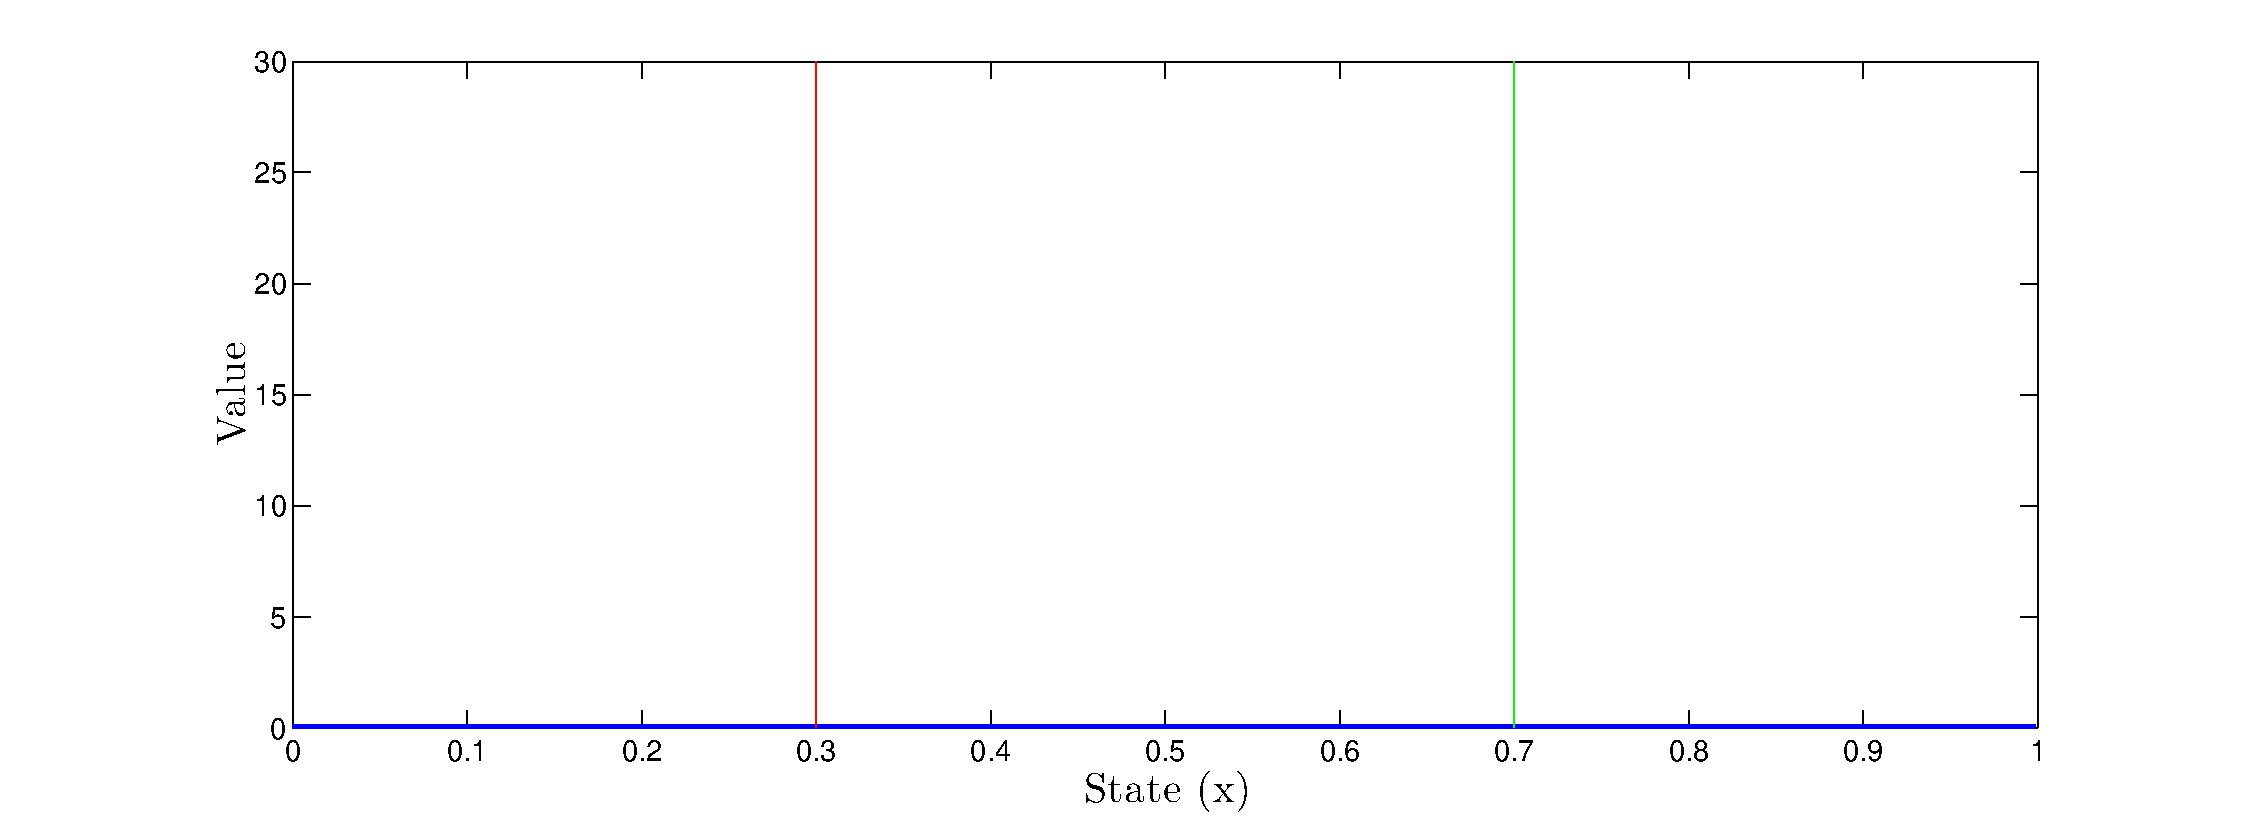
\includegraphics[width=260pt]{smp_sym.pdf}
\caption{Symmetric rewards.}
\label{fig:smpasmreward1}
\end{subfigure}

\begin{subfigure}[b]{0.5\textwidth}
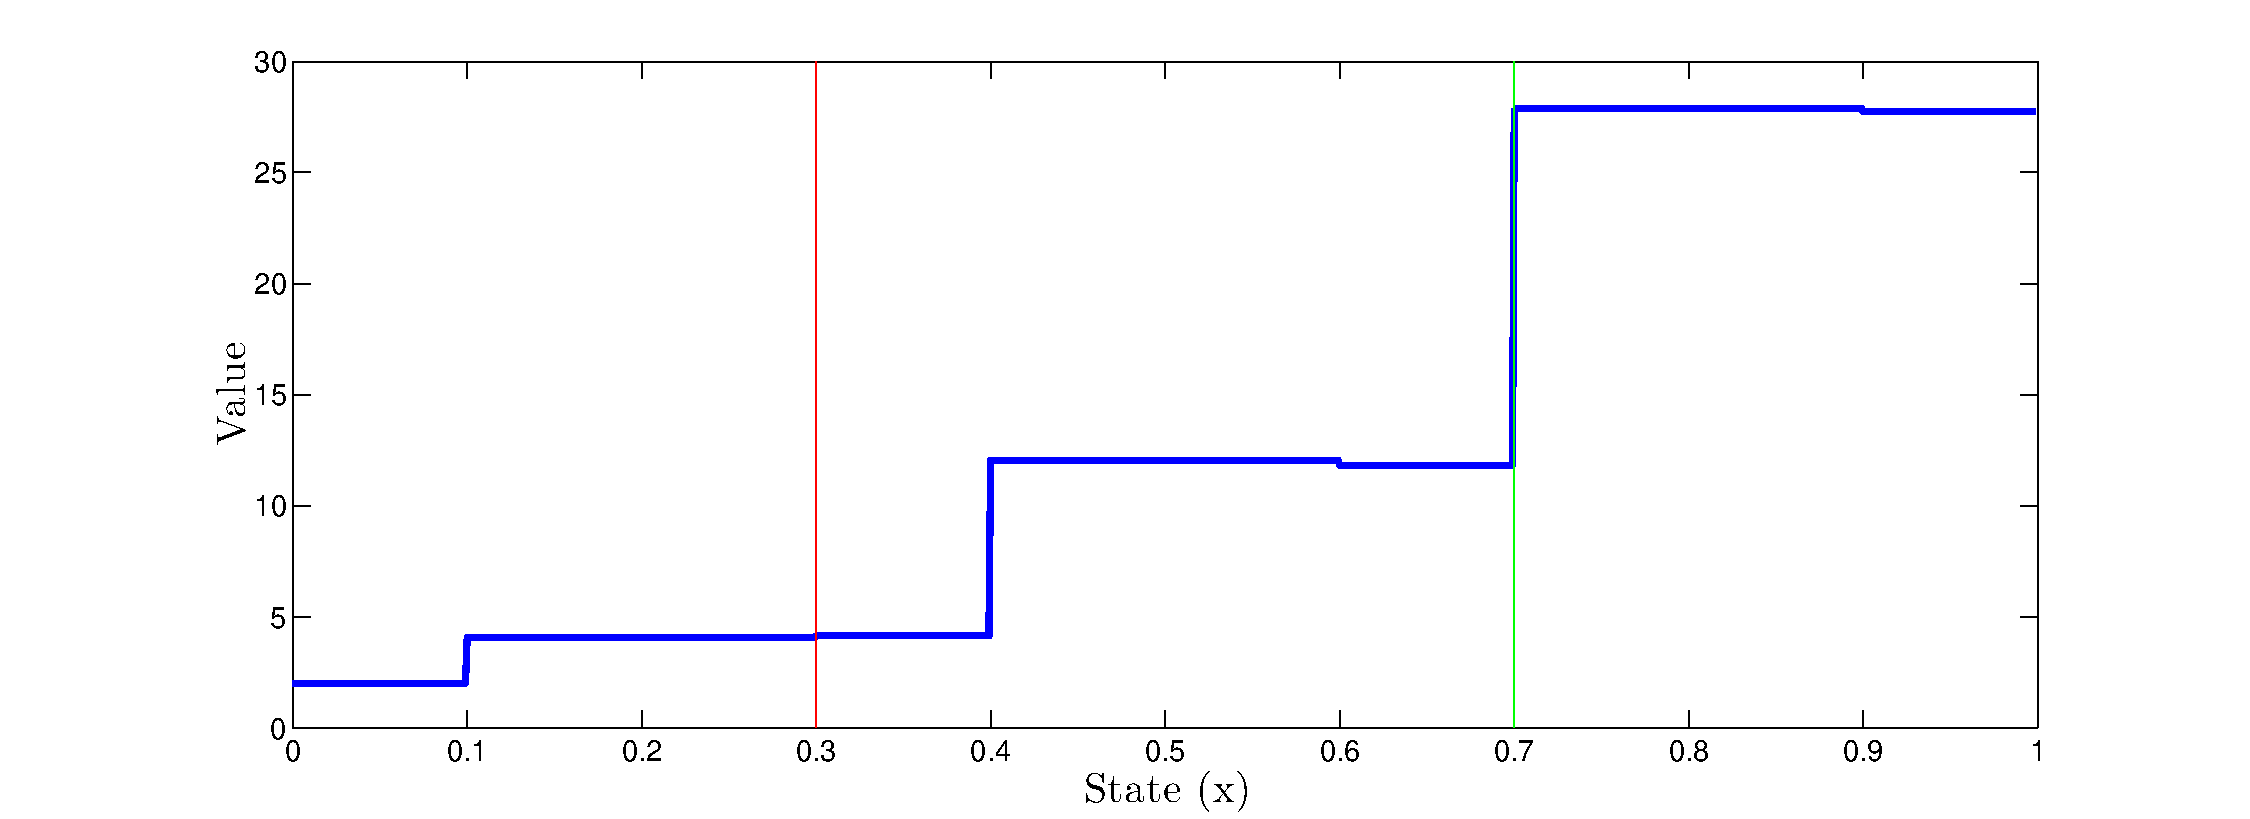
\includegraphics[width=260pt]{smp_asym.pdf}
\caption{Asymmetric rewards.}
\label{fig:smpasmreward2}
\end{subfigure}

\vspace{-2mm}
\caption{Optimal value functions for continuous stochastic matching 
            pennies under (a) symmetric and (b) asymmetric reward 
            structures at horizon 4. Threshold values $c$ 
            and $d$ are highlighted in red and green, respectively. 
            The step size is $k = 0.3$.}
\label{fig:smpasmreward}
\end{figure}

Figure \ref{fig:smpasmreward1} shows the results of the continuous
stochastic matching pennies game using the symmetric reward structure
given in Table \ref{tab:smpsymreward}. 
The results show that the expected reward for Player 1 remains at zero
over all 4 horizons, irrespective of the state $x$. Given the symmetric
rewards in each region, both players are indifferent between their 
pure strategies. Hence, the expected reward for each player is zero in
all regions. This corresponds to the well known solution of the 
matching pennies game where the rewards are symmetric and serves 
as a proof of concept for our novel solution technique.

The effect of the asymmetric reward structure, given in Table \ref{tab:smpasymreward}, 
is shown in Figure \ref{fig:smpasmreward2}. From the figure it is clear that Player 1 achieves the highest expected
reward in Region 3, followed by Region 2 and finally by Region 1. This
is to be expected given the nature of the asymmetric rewards within
each region. The results indicate that the two players are
no longer indifferent between their pure strategies in each region. 

\subsection{Binary Option Stochastic Game}

Binary options are financial instruments which allow an investor to
bet on the outcome of a yes/no proposition. The proposition typically
relates to whether the price of a particular asset that underlies the option
will rise above or fall below a specified amount, known as the strike
price, $\kappa \in \mathbb{R}$. When the option reaches maturity the 
investor receives a fixed pay-off if their bet was correct and nothing otherwise.

\subsubsection{Domain Description}

We analyse the valuation of a binary option as an extensive form
zero-sum game between a trader and the market. The aim of the trader
is to maximise their expected discounted pay-off at a fixed horizon $H$ 
through buying and selling options within an adversarial market. 
The problem has two state variables: the underlying market value of the option
$v \in [0, 100]$ and the trader's inventory of options $i \in \mathbb{N}$.

At each time step the trader can execute one of three actions
$a_{trd} \in \left\{buy_{trd}, sell_{trd}, hold_{trd}\right\}$, where $buy_{trd}$ refers to a request to 
buy an option from the market, $sell_{trd}$ refers to a request to sell an option to
the market and $hold_{trd}$ is equivalent to taking no action. 
The market can execute one of two actions: $a_{mkt} \in \left\{sell_{mkt}, nsell_{mkt} \right\}$,
where $sell_{mkt}$ corresponds to selling an option to the trader and $nsell_{mkt}$ 
corresponds to not selling to the trader. 

The joint actions of the trader and market, $a_{\text{trd}}$ and 
$a_{\text{mkt}}$, respectively, affect both the market value of the option
and the trader's inventory. For the sake of simplicity we assume that
the market value may increase or decrease by fixed step sizes, 
$u \in \mathbb{R}$ for an increase and $d \in \mathbb{R}$ for a decrease.

The trader's option inventory dynamics are given by:

{\small 
\abovedisplayshortskip=0pt
\belowdisplayshortskip=0pt
\begin{equation*}
P(i' | v, i, a_{\text{trd}}, a_{\text{mkt}}) = \delta \left[ i' - \begin{cases}
      (buy_{trd}) \wedge (sell_{mkt}) : & i + 1 \\ 
      (sell_{trd}) \wedge (i > 0) : & i - 1 \\
      otherwise: & i \\
    \end{cases} \right] \\
\end{equation*}
}%

It should be noted that under this formulation the market will always
buy an option from the trader when the trader selects $sell_{trd}$. 
The market value changes according to:

{\small 
\abovedisplayskip=0pt
\belowdisplayskip=0pt
\begin{align*}
P(v' | v, i, a_{\text{trd}}, a_{\text{mkt}}) &= \\
&
\delta \left[ v' - \begin{cases}
      (buy_{trd}) \wedge (sell_{mkt})  : & v + u \\
       (sell_{trd}) \wedge (i > 0) : & v - d \\
      otherwise: & v
    \end{cases} \right] & \\    
\end{align*}
}%

%The market value of the option is contingent upon the actions of the
%trader and a Bernoulli distributed random variable, $\epsilon \sim \text{Bernoulli}(p)$, 
%where $p \in [0, 1]$. By varying the parameter $p$ the latent market
%dynamics can be made to approximate a bull or bear market.

Assuming that the strike price $\kappa \in [0, 100]$, the rewards obtained by the trader are given by:
{\small 
\begin{equation}
  R_{trader} = 
    \begin{cases}
      (sell_{trd}) \wedge (i > 0) \wedge (v > \kappa) : & 1 \\ 
      otherwise : & 0 \\
    \end{cases} \nonumber
\end{equation}
}%

The market's reward is simply the additive inverse of the trader's 
reward. Hence, the binary option game is zero-sum. 

\subsubsection{Results}

%%%%%%%%%%%%%%%%%%%%%%%%%%%%%%%%%
% Figure
%%%%%%%%%%%%%%%%%%%%%%%%%%%%%%%%%

\begin{figure}[h!]
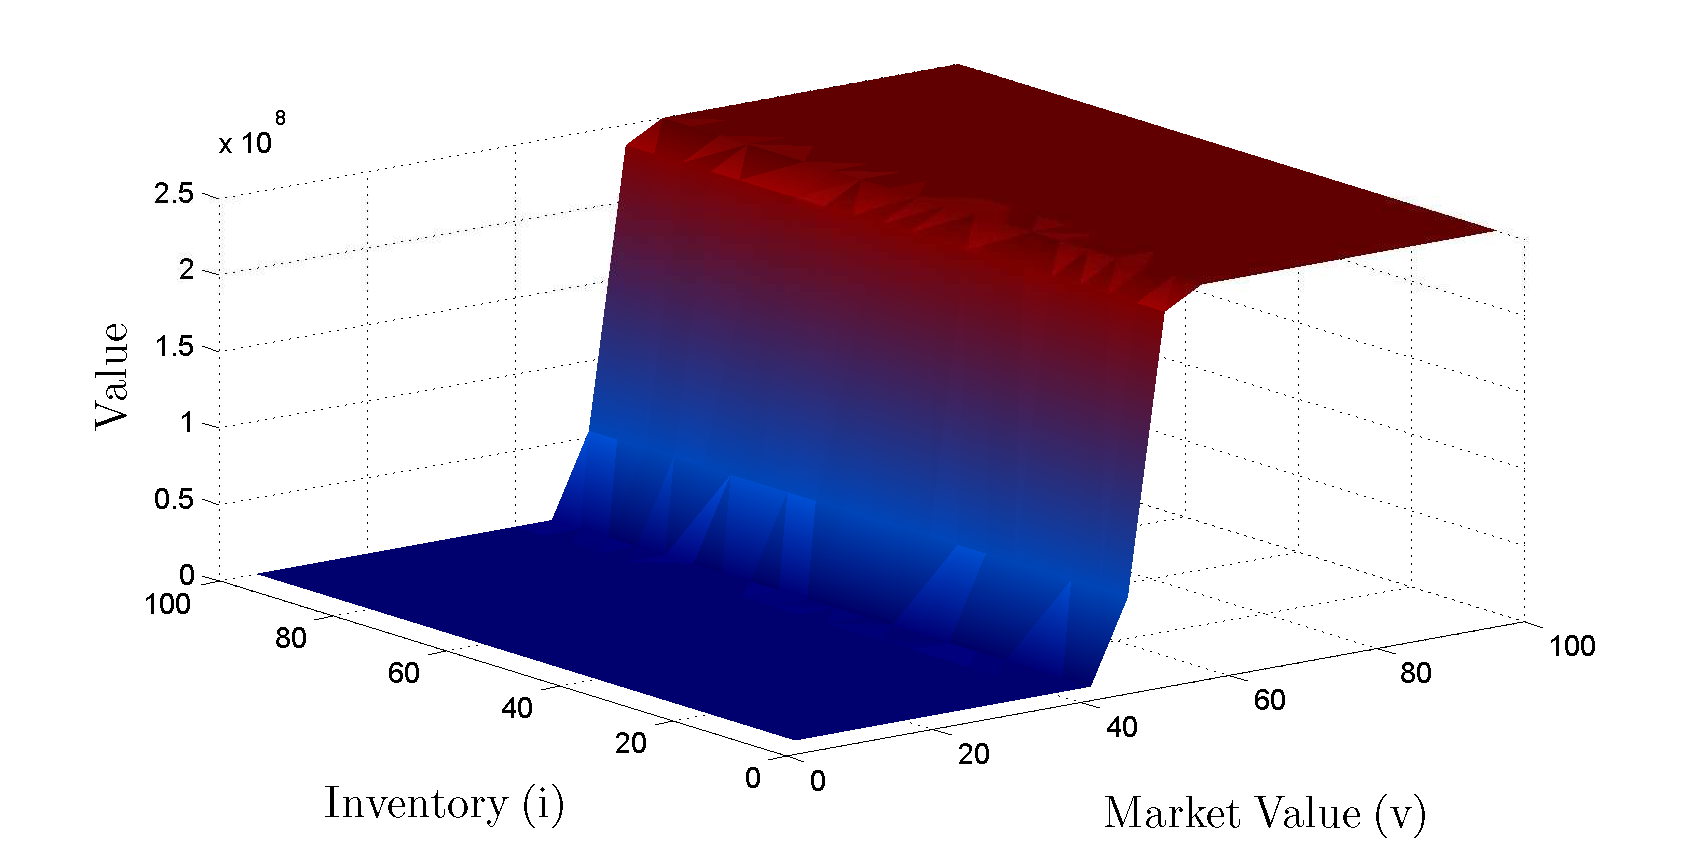
\includegraphics[width=250pt]{sbo.pdf}
\vspace{-3mm}
\caption{The optimal value function for the binary option game at horizon 20. The strike price is set to $\kappa = 45.0$ and the increment and
decrement values are set to $u = 1.0$ and $d = 1.0$, respectively.}
\label{fig:binaryoptionvfunc}
\end{figure}

In Figure \ref{fig:binaryoptionvfunc} we show the optimal value function for the
binary option game at horizon 20. The strike price $\kappa = 45.0$ and
the increment and decrement values, $u$ and $d$ are both set to 1.0. The
value function clearly shows that under this formulation the trader
achieves the most reward by selling the option as soon $v > \kappa$.
Selling an option triggers the underlying value to decrease, which triggers
the trader to buy once the value falls beneath the strike price. This leads
to the continual cycling of buying and selling of the option at values close
to the strike price $\kappa$. In essence the trader behaves like a market
maker in that they take both sides of the transaction at values near 
$\kappa$.

\subsection{Robust Energy Production}

The provision of energy resources is an integral component of any
economy. Energy providers must be able to produce energy in response
to changes in energy demand. In situations where demand exceeds supply,
an energy crises may occur. In this paper we investigate energy 
production from the viewpoint of an energy provider responsible for 
supplying energy in an adversarial environment.

\subsubsection{Domain Description}

We define our energy production domain as an extensive form zero-sum
game between an energy provider and nature. The aim of the energy
provider is to maximise its expected discounted reward at a 
fixed horizon $H$ by changing production levels in response to changes in demand.
The domain has two state variables: the production level $p \in \mathbb{R}$ and the energy demand
$d \in \mathbb{R}$. 

At each time step the energy provider can execute one of two actions
$a_{prd} \in \left\{dec_{prd}, inc_{prd}\right\}$, where $dec_{prd}$ 
refers to increasing energy production and $inc_{prd}$ refers to decreasing
energy production. Nature can also execute one of two actions
$a_{nat} \in \left\{dec_{nat}, inc_{nat}\right\}$, where $dec_{nat}$ 
refers to increasing energy demand and $inc_{nat}$ refers to decreasing
energy demand. For $i \in \left\{prd, nat\right\}$ we restrict 
$\left\{dec_i, inc_i\right\} \in \mathbb{Z}$.

The joint actions of the energy provider and nature, $a_{prd}$ and
$a_{mkt}$, respectively, affect the production level as follows:

{\small 
\abovedisplayskip=0pt
\belowdisplayskip=0pt
\begin{align*}
&P(p' | d, p, a_{\text{prd}}, a_{\text{nat}}) = \\
\\
& \hspace{40pt} \delta \left[ p' - \begin{cases}
      (inc_{prd})  : & p + inc_{prd} \\
       (dec_{prd}) \wedge (p > dec_{prd}): & p - dec_{prd} \\
      otherwise: & p
    \end{cases} \right] & \\    
\end{align*}
}%

The energy demand changes according to:
{\small 
\abovedisplayskip=15pt
\belowdisplayskip=0pt
\begin{align*}
&P(d' | d, p, a_{\text{prd}}, a_{\text{nat}}) = \\
\\
& \hspace{40pt}\delta \left[ d' - \begin{cases}
      (inc_{nat})  : & d + inc_{nat} \\
       (dec_{nat}) \wedge (d > dec_{nat}) : & d - dec_{nat} \\
      otherwise: & d
    \end{cases} \right] & \\    
\end{align*}
}%

The reward obtained by the energy provider are specified as:

\vspace{-1.5mm}
{\small 
\abovedisplayshortskip=0pt
\belowdisplayshortskip=0pt
\begin{equation}
  R_{prd} = 
    \begin{cases}
      (p < d) : & -100 \\ 
      otherwise : & 0 \\ 
    \end{cases} \nonumber
\end{equation}
}%

We note that under this reward structure not meeting energy demand
is heavily penalised, whereas meeting or even exceeding demand are
given the same reward. Nature's reward is simply the additive inverse 
of the energy provider's reward.

\subsubsection{Results}

%%%%%%%%%%%%%%%%%%%%%%%%%%%%%%%%%
% Figure
%%%%%%%%%%%%%%%%%%%%%%%%%%%%%%%%%

\begin{figure}[ht!]
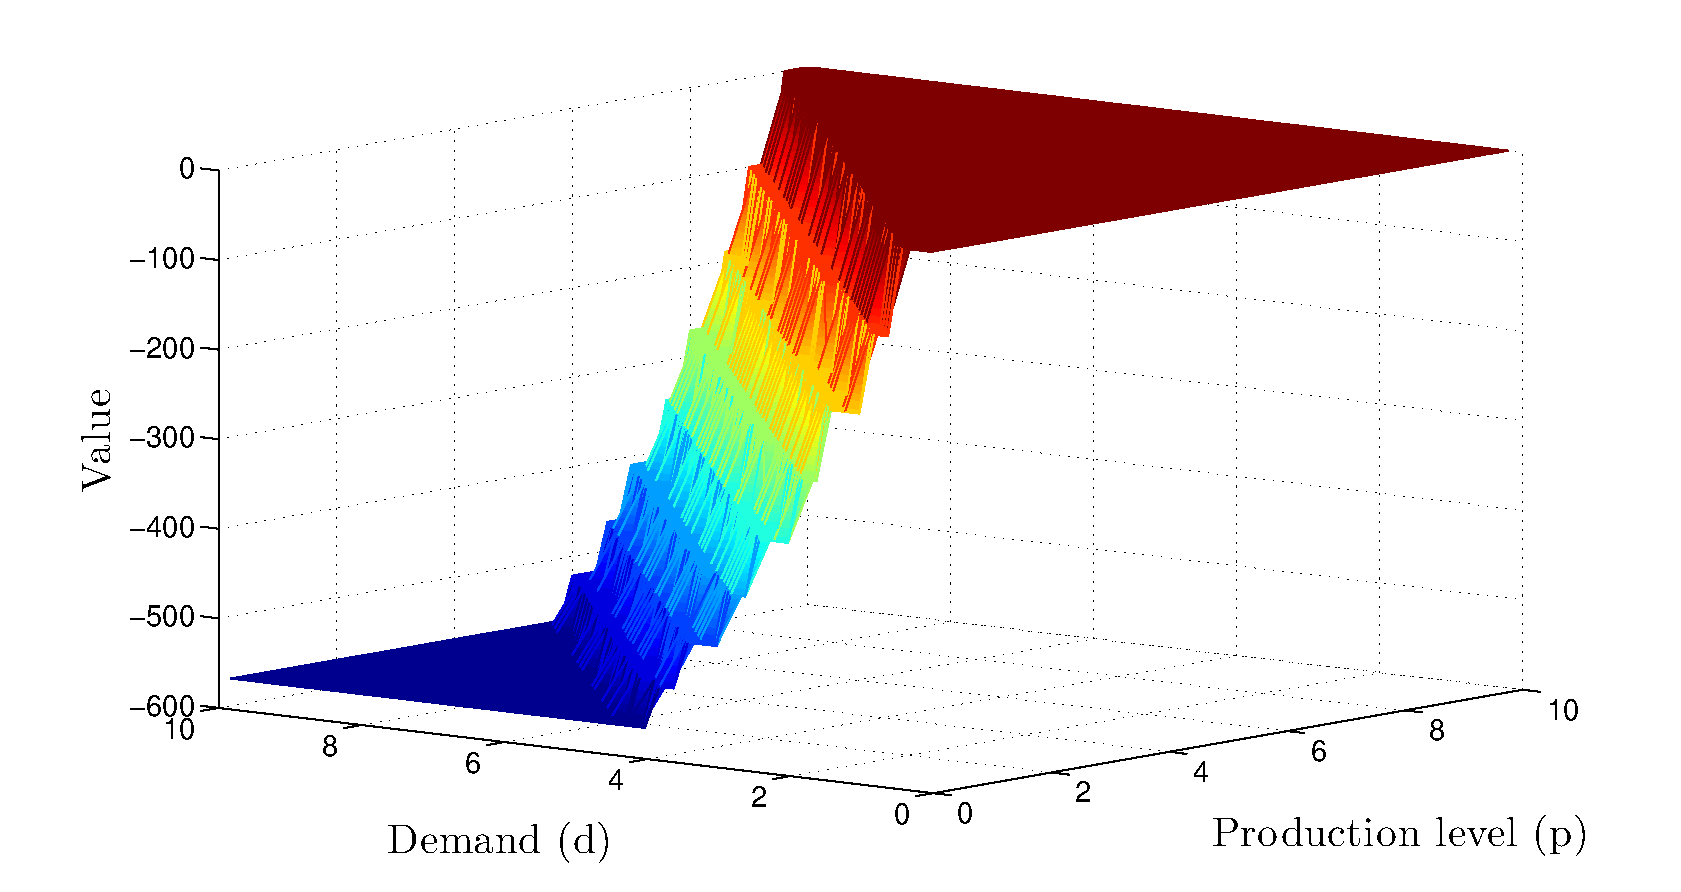
\includegraphics[width=250pt]{sep.pdf}
\vspace{-3mm}
\caption{The optimal value function for the robust energy production game at horizon 8. 
The increase and decrease variables where set to $dec_{prd} = inc_{prd} = 1.0$ and $dec_{nat} = inc_{nat} = 0.5$, respectively.}
\label{fig:sepvfunc}
\end{figure}

%%%%%%%%%%%%%%%%%%%%%%%%%%%%%%%%%

In Figure \ref{fig:sepvfunc} we show the optimal value function
for the robust energy production game at horizon 8. The value
function shows that the highest value is attained when the energy provided
exceeds demand. This is clearly evident given the nature of the reward structure.
When the demand exceeds the amount produced, the value is at its lowest.
Here we note that the value function decreases in a step-wise manner
from the point where where production level meets demand. This indicates
that production levels just beneath demand have a higher value than
those well below demand.


%-----------------------------------------------------------------------------
% Related Work 
%-----------------------------------------------------------------------------

\section{Related Work}
\label{sec:relatedwork}

Solutions to stochastic games have been proposed from within both
game theory and reinforcement learning. The first algorithm, game theoretic or otherwise, for 
finding a solution to a stochastic game was given by Shapley \cite{Shapley_PotNAoS_1953}.
The algorithm repeatedly calculates a value function $V(s)$ over discrete states
which converges to an optimal value function $V^{*}(s)$, which represents
the expected discounted future reward if both players in the game followed
the game's Nash equilibrium. Shapley's algorithm is in essence an 
extension of the value iteration algorithm to stochastic games. 

A reinforcement 
learning based solution to stochastic games was first introduced by 
\cite{Littman_ICML_1994}. Littman's algorithm, Minimax-Q,
extends the traditional Q-learning algorithm for MDPs to 
zero-sum discrete stochastic games. The algorithm converges to the 
stochastic game's equilibrium solution. Hu and Wellman \cite{Hu_ICML_1998}
extended Minimax-Q to general-sum games and proved that it converges
to a Nash equilibrium under certain restrictive conditions. Although
both reinforcement learning based algorithms are able to calculate 
equilibrium solutions they are limited to discrete state formulations of
stochastic games. In this paper we calculate exact solutions to 
continuous state formulations of stochastic games, under certain restrictions.
The Dec-MDP \cite{Bernstein_MoOR_2002} framework allows
for decentralised control within continuous state spaces but is limited
to general-sum systems. In this paper we provide the first 
known exact closed-form solution to a subclass of continuous state zero-sum 
stochastic games defined by a piecewise constant reward and piecewise linear transition.

Several techniques have been put forward to tackle continuous state
spaces in MDPs. Li and Littman \cite{Li_AAAI_2005} describe a method
for approximate solutions to continuous
state MDPs.  In their work, Li and Littman only allow for rectilinearly aligned 
constraints in their reward and transition functions (not arbitrary linear constraints)
and cannot handle general linear transition models without approximation.  
Our SDP method provides exact solutions without these restrictions, which
makes SDP strictly more general.  Also, Li and Littman did not consider 
game-theoretic extensions of their work or the parameterised optimisation 
problem that these extensions entail.

Symbolic dynamic programming techniques have been previously used to
calculate exact solutions to single agent MDPs with both continuous
state and actions in a variety of non-game theoretic domains
\cite{Sanner_UAI_2011,Zamani_AAAI_2012}.  In this paper we build on
this work and present the first application of SDP to stochastic games
with concurrently acting agents.

%----------------------------------------------------------------------------
%The use of reinforcement learning methods to solve stochastic games
%was introduced by Littman \cite{Littman_ICML_1994}. Under Littman's
%formulation optimal policies can be calculated for discrete state zero-sum 
%stochastic games using an algorithm akin to Q-learning. Hu \cite{Hu_ICML_1998}
%extended Littman's framework into the general-sum case. Whilst both
%approaches provide optimal policies for stochastic games under zero-sum
%and general sum settings, they are limited to discrete state formulations. 
%
%A lazy approximation technique for MDPs which imposes similar restrictions on the
%form of the reward and transition functions was introduced by Li \cite{Li_AAAI_2005}
%and allows for the calculation of approximate solutions. Our approach using
%symbolic dynamic programming calculates exact solutions in game theoretic
%settings. 







%-----------------------------------------------------------------------------
% Conclusions and Future Work
%-----------------------------------------------------------------------------

\label{sec:conclusion}

% implications of decisions, possibility of extension

% while not scalable for 100's of items, these represent
% the first general exact solution methods for capacitated
% multi-inventory control problems

% have to define exact solution and understand properties
% before proceeding to approximate as an extension of this
% work

% bilinear issues

% quadratic quite limited but useful for single continuous
% resource or continuous time

% symbolic constrained optimization -- other uses

% Future work:
%
% - Application to Inventory (makes clear that there are
%     simplifications possible in current solution), consider
%     submitting to CPAIOR, Informs?
% - Exponential Distribution for Stochasticity?
% - Parameterized linear programming, application to graphical
%     models or efficient LP solutions, MAP Bayesian approaches
%     for uniforms?
% - Affine XADD, useful for mixture of uniforms in Bayesian work.
% - Efficient linear programming -- exploiting factorized
%     structure in constraints using variable elimination
% - Symbolic Policy Iteration for CSA-MDPs (good for Inventory,
%     what other problems that have a simple policy?  Traffic?)
% - Theoretical guarantees on (linear) XADD (minimal function, 
%     canonical?)  Efficient LADD implementation.  Quadratic
%     linearization would need to come in max step.  Pruning
%     inside the LADD... implement feasibility checking.
% - Nonlinear solutions (can we solve any more expressive problems?)
% - Approximation
%   * adaptively linearize the problem (especially for nonlinear, 
%     bilinear)
%   * XADD approximation?  Othogonal polynomials?

We have presented an SDP solution for continuous state \emph{and}
action MDPs with the key contribution of \emph{symbolic constrained
optimization} to solve the continuous action maximization problem.  We
believe this is the first work to propose optimal closed-form
solutions to MDPs with \emph{multivariate} continuous state \emph{and}
actions, discrete noise, \emph{piecewise} linear dynamics, and
\emph{piecewise} linear (or restricted \emph{piecewise} quadratic)
reward; further, we believe our experimental results are the first
exact solutions to these problems to provide a closed-form optimal
policy for all (continuous) states.



%-----------------------------------------------------------------------------
% Bibliography
%-----------------------------------------------------------------------------

%\bibliographystyle{plain}
\bibliographystyle{authordate1}
\bibliography{uai2014}

\end{document}
